\documentclass[mathserif, handout]{beamer}
\usepackage{url}
% ======================================================================
% General LaTeX Setup for Beamer (Reusable Preamble)
% Author: Chandra Gummaluru
% ======================================================================

\documentclass[mathserif, handout]{beamer}
\setbeamertemplate{frametitle}{}

% ------------------------------------------------------------
% basic packages
% ------------------------------------------------------------
\usepackage{url}
\usepackage{ifthen}
\usepackage{enumerate}
\usepackage[font=small]{caption}
\usepackage{subcaption}
\usepackage{moresize}
\usepackage[outline]{contour}
\usepackage{transparent}
\usepackage{worldflags}
\usepackage{bm}
\usepackage{graphbox}
\usepackage{mathtools}
\usepackage{multirow}
\usepackage{fontawesome5}
\usepackage{pifont}
\usepackage{array}
\usepackage{comment}

% ------------------------------------------------------------
% math
% ------------------------------------------------------------
\DeclarePairedDelimiter{\floor}{\lfloor}{\rfloor}
\DeclarePairedDelimiter{\ceil}{\lceil}{\rceil}

% ------------------------------------------------------------
% colors
% ------------------------------------------------------------
\definecolor{hl}{RGB}{248,196,69}
\definecolor{myred}{HTML}{ED5565}
\definecolor{myorange}{HTML}{FC6E51}
\definecolor{myyellow}{HTML}{FFCE54}
\definecolor{mycyan}{HTML}{4FC1E9}
\definecolor{myblue}{HTML}{5D9CEC}

\newcommand{\graytext}[1]{\footnotesize\color{gray}#1\normalsize\color{black}}

% ------------------------------------------------------------
% symbols
% ------------------------------------------------------------
\newcommand{\cmark}{\ding{51}}
\newcommand{\xmark}{\ding{55}}

% ------------------------------------------------------------
% highlighting
% ------------------------------------------------------------
\newcommand{\reducedstrut}{\vrule width 0pt height .9\ht\strutbox depth .9\dp\strutbox\relax}
\newcommand{\highlight}[1]{%
  \begingroup\setlength{\fboxsep}{0pt}\colorbox{hl}{\reducedstrut$\displaystyle #1$\/}\endgroup}
\newcommand{\highlightc}[2]{%
  \begingroup\setlength{\fboxsep}{0pt}\colorbox{#1}{\reducedstrut$\displaystyle #2$\/}\endgroup}

% ------------------------------------------------------------
% environments (boxes)
% ------------------------------------------------------------
\usepackage{tcolorbox}
\tcbuselibrary{skins}

\newtcolorbox{thmbox}[1][]{colback=gray!30!white!20, colframe=black, fonttitle=\bfseries, title=#1, boxrule=0.5pt}

% 1) Bottom open (draw top + sides only)
\newtcolorbox{thmboxtop}[1][]{
    enhanced,
    frame hidden,
    colback=gray!30!white!20,
    borderline north={0.5pt}{0pt}{black}, % top
    borderline west={0.5pt}{0pt}{black},  % left
    borderline east={0.5pt}{0pt}{black}   % right
}

% 2) Top open (draw bottom + sides only)
\newtcolorbox{thmboxbot}[1][]{
    enhanced,
    frame hidden,
    colback=gray!30!white!20,
    borderline south={0.5pt}{0pt}{black}, % bottom
    borderline west={0.5pt}{0pt}{black},  % left
    borderline east={0.5pt}{0pt}{black}   % right
}

% 3) Side only (draw only left and right)
\newtcolorbox{thmboxside}[1][]{
    enhanced,
    frame hidden,
    colback=gray!30!white!20,
    borderline west={0.5pt}{0pt}{black},  % left
    borderline east={0.5pt}{0pt}{black}   % right
}

\newtcolorbox{defboxtop}[1][]{
    enhanced,
    colback=gray!30!white!20,
    frame hidden,
    overlay={
        % Draw top + sides with rounded corners
        \draw[line width=0.5pt, black, rounded corners=3mm]
            (frame.south west) -- (frame.north west) -- (frame.north east) -- (frame.south east);
    },
    #1
}

\newtcolorbox{defboxbot}[1][]{
    enhanced,
    colback=gray!30!white!20,
    frame hidden,
    overlay={
        % Draw top + sides with rounded corners
        \draw[line width=0.5pt, black, rounded corners=3mm]
            (frame.north west) -- (frame.south west) -- (frame.south east) -- (frame.north east);
    },
    #1
}

\newtcolorbox{defboxside}[1][]{
    enhanced,
    frame hidden,
    colback=gray!30!white!20,
    borderline west={0.5pt}{0pt}{black},  % left
    borderline east={0.5pt}{0pt}{black}   % right
}

\newtcolorbox{proofbox}[1][]{colback=gray!20!white!20, colframe=grey, fonttitle=\bfseries, title=#1, boxrule=0.5pt, colbacktitle=white, enhanced jigsaw, sharp corners}

% ------------------------------------------------------------
% code listings
% ------------------------------------------------------------
\usepackage{listings}
\lstdefinestyle{mypython}{
  language=Python,
  deletekeywords=[2]{open, next, from, chr, str, int},
  morekeywords=[3]{List, Graph, Tree, Dict, Set, UnionFind, Ordict, Trie, Queue},
  morekeywords=[4]{ListNode, Vertex, Edge, Path, TreeNode, DictNode, UnifNode, OrdictNode, TrieNode, QueueNode},
  morekeywords=[5]{True, False, Boolean, String, Integer, Key, Function, KeyedObject, Object, Array, Tuple, Optional, None},
  keywordstyle=\color{mycyan}\bfseries,
  keywordstyle=[3]\color{myblue}\bfseries,
keywordstyle=[4]\color{myblue}\bfseries,
keywordstyle=[5]\color{mycyan}\bfseries,
  stringstyle=\color{orange},
  commentstyle=\color{gray}\itshape,
  basicstyle=\ttfamily\footnotesize,
  numbers=left,
  numberstyle=\tiny\color{gray},
  stepnumber=1,
  numbersep=5pt,
  xleftmargin=15pt,
  frame=none,
  showstringspaces=false,
  breaklines=true,
  breakatwhitespace=true,
  tabsize=4,
  columns=flexible
}


% ------------------------------------------------------------
% algorithms
% ------------------------------------------------------------
\usepackage{algorithm}
\usepackage[endLComment=~]{algpseudocodex}
\makeatletter
\algrenewcommand\ALG@beginalgorithmic{\footnotesize}
\makeatother

% ------------------------------------------------------------
% optimization environments
% ------------------------------------------------------------
\usepackage[nocomma]{optidef}

% ------------------------------------------------------------
% pgfplots and pie charts
% ------------------------------------------------------------
\usepackage{pgfplots}
\usepackage{pgf-pie}
\pgfplotsset{compat=1.7}

% ------------------------------------------------------------
% tikz
% ------------------------------------------------------------
\usepackage{tikz}
\usetikzlibrary{
  angles, quotes, positioning, fit, backgrounds, shapes.geometric, intersections,
  calc, shapes, mindmap, decorations.text, arrows, arrows.meta,
  automata, chains, decorations.pathreplacing, calligraphy,
  decorations.markings, shapes.misc, decorations.pathmorphing
}
\tikzset{
  invisible/.style={opacity=0},
  visible on/.style={alt=#1{}{invisible}},
  alt/.code args={<#1>#2#3}{\alt<#1>{\pgfprioritysalso{#2}}{\pgfprioritysalso{#3}}}
}

\newcommand{\multiedge}[5][]{
\pgfmathsetmacro{\N}{#4}
\pgfmathsetmacro{\mid}{(\N-1)/2}
\foreach \i in {0,...,\numexpr#4-1\relax} {

\pgfmathsetmacro{\k}{\i-\mid}
\draw[#1] ($ (#2) + \k*#5*($(#2)!1!90:(#3)$) $) -- ($ (#3) + \k*#5*($(#2)!1!90:(#3)$) $); 

}
\draw[#1,  -{>[scale=1]}]
  ($(#2)!0.54!(#3)$) -- ($(#2)!0.55!(#3)$);
}

% ------------------------------------------------------------
% bibliography
% ------------------------------------------------------------
\usepackage[style=ieee]{biblatex}
\setbeamertemplate{bibliography item}{\insertbiblabel}
\setbeamertemplate{background canvas}{
  \begin{tikzpicture}[remember picture,overlay]
    \node[opacity=0.0075]
      at (current page.center)
      {
\includegraphics[width=0.8\paperwidth]{images/signature.pdf}};
  \end{tikzpicture}
}

% ------------------------------------------------------------
% beamer theme and settings
% ------------------------------------------------------------
\usetheme{Boadilla}
\usecolortheme{seagull}
\beamertemplatenavigationsymbolsempty
\setbeamertemplate{enumerate item}{(\arabic{enumi})}
\setbeamertemplate{enumerate subitem}{(\alph{enumii})}
\setbeamertemplate{enumerate subsubitem}{(\roman{enumiii})}
\setbeamertemplate{itemize item}[circle]
\setbeamertemplate{itemize subitem}{\circ}
\setbeamertemplate{itemize subsubitem}{-}
\setbeamercolor{item}{fg=black!40}
\setbeamercovered{transparent=10}

% ===========================
% Premade TikZ Figure Commands
% ===========================

% images w/ labels
% inside tikz as a node
\NewDocumentCommand{\labeledimgnodetikz}{O{} m m m m m m}{%
	\begin{scope}[transparency group, #1]
		\node[
			draw,
			circle,
			inner sep=0,
			outer sep=0,
			minimum size=10mm,
			#1
		] (#5) at (#3,#4)
		{\includegraphics[scale=#7]{#6}};
		\node[
			rectangle,
			draw=black,
			thick,
			fill=black!55,
			rounded corners=0.1mm,
			inner sep=0pt,
			outer sep=0pt,
			minimum size=2.8mm,
			minimum width=3.5mm
		] at (#3,#4-0.1) {};
		\node[outer sep=0, inner sep=0, white] at (#3,#4-0.1) {\footnotesize #2};
	\end{scope}
}

% inside tikz isolated

% outside tikz
\NewDocumentCommand{\labelednode}{m}{%
	\begin{tikzpicture}[baseline={(0,-1mm)}]
		\node[
			rectangle,
			thick,
			draw=black,
			fill=black!55,
			rounded corners=0.1mm,
			inner sep=0pt,
			outer sep=0pt,
			minimum size=2.8mm,
			minimum width=3.5mm
		] at (0,0) {};
		\node[outer sep=0, inner sep=0, white, minimum size=2.8mm, minimum width=3.5mm] at (0,0) {\footnotesize #1};
	\end{tikzpicture}
}

% images only
% inside tikz as a node
\NewDocumentCommand{\imgnodetikz}{O{} m m m m m m}{%
	\begin{scope}[transparency group, #1]
		\node[
			draw,
			circle,
			inner sep=0,
			outer sep=0,
			minimum size=10mm,
			#1
		] (#5) at (#3,#4)
		{\includegraphics[scale=#7]{#6}};
		\node[
			rectangle,
			draw,
			thick,
			fill=black!55,
			rounded corners=0.1mm,
			inner sep=0pt,
			outer sep=0pt,
			minimum size=2.8mm,
			minimum width=3.5mm,
			opacity=0
		] at (0,0) {};
		\node[outer sep=0, inner sep=0, white, opacity=0] at (0,0) {\footnotesize #2};
	\end{scope}
}

% inside tikz isolated
\NewDocumentCommand{\imgtikz}{O{} mm}{%
	\begin{scope}[transparency group, #1]
		\node[
			inner sep=0,
			outer sep=0
		] (#5) at (#3,#4)
		{\includegraphics[scale=#3]{#2}};
	\end{scope}
}


% outside tikz
\NewDocumentCommand{\imgnode}{mm}{%
	\begin{tikzpicture}[baseline={(0,-1mm)}]
        \node[
            inner sep=0,
            outer sep=0,
            draw opacity=0,
        ] at (0,0)
        {\includegraphics[scale=#2]{#1}};
    \end{tikzpicture}
}

% outside tikz (inline)
\newcommand{\imgnodetext}[2]{%
	\hspace{-0.5mm}%
	\raisebox{-0.26\height}{%
		\includegraphics[scale=#2]{#1}%
	}%
	\hspace{-0.5mm}%
}


% labels only
% inside tikz as a node
\NewDocumentCommand{\labeltikz}{m}{%
	\node[
		rectangle,
		thick,
		draw=black,
		fill=black!55,
		rounded corners=0.1mm,
		inner sep=0pt,
		outer sep=0pt,
		minimum size=2.8mm,
		minimum width=3.5mm
	] at (0,0) {};
	\node[outer sep=0, inner sep=0, white, draw opacity=0] at (0,0) {\footnotesize #1};
}

% inside tikz isolated

% outside tikz

% === define custom pgfkeys ===
\pgfkeys{
	/devicenode/.is family, /devicenode,
	outline thickness/.initial=thick,
	outline color/.initial=black
}

\NewDocumentCommand{\qpacket}{m}{%
	\begin{tikzpicture}[baseline=(current bounding box.center)]
		\node at (0.5,0.4) {\includegraphics[scale=0.1]{#1}};
	\end{tikzpicture}%
}

\NewDocumentCommand{\bpacketid}{mmm}{%
	\begin{tikzpicture}[baseline=(current bounding box.center)]
		\begin{scope}[shift={(0.85,0.7)}]
			\draw[thick, draw=black, fill=#1, rounded corners=1pt] (0.01,0.05) rectangle node[white, text width=1cm, align=center] {\color{#3}\footnotesize #2} (-0.71,-0.625);
		\end{scope}
	\end{tikzpicture}%
}

\NewDocumentCommand{\packetid}{mmmm}{%
	\begin{tikzpicture}[baseline=(current bounding box.center)]
		\begin{scope}[shift={(0.85,0.7)}]
			\draw[thick, draw=black, fill=#2, rounded corners=1pt] (0.01,0.05) rectangle node[white, text width=1cm, align=center] {\color{#4}\footnotesize #3} (-0.71,-0.625);
			\node[
				star,
				star points=30,
				star point ratio=0,
				scale=1.5,
				draw=black,
				thick,
				fill=white,
				rounded corners=0.1mm,
				inner sep=0pt,
				minimum size=2.8mm
			] at (0,0) {};
			\node at (0,0) {\footnotesize #1};
		\end{scope}
	\end{tikzpicture}%
}

\tikzset{
	dictnode/.pic={
			\draw[thick, fill=#1, line join=]
			(-0.75,-0.5) --
			(-0.75,0.5)  --
			(0.75,0.5) --
			(0.75,-0.5) --
			cycle --
			(-0.75, 0.75) --
			(0.75, 0.75) --
			(0.75, -0.5) --
			cycle;
		}
}

\tikzset{
	queuenode/.pic={
			\draw[thick, fill=#1, line join=round]
			(-0.85,-0.5) --
			(-0.85,0.5)  --
			(0.65,0.5) --
			(0.75,0) --
			(0.65,-0.5) --
			cycle;
		}
}

\tikzset{
	queuenodetail/.pic={
			\draw[thick, fill=#1, line join=round]
			(-0.75,-0.5) --
			(-0.75,0.5)  --
			(0.65,0.5) --
			(0.75,0) --
			(0.65,-0.5) --
			cycle;
		}
}

\tikzset{
	listnode/.style={
			shape=rectangle,
			rounded corners,
			thick,
			minimum height=10mm,
			minimum width=15mm,
			inner sep=0pt
		}
}

\tikzset{
	arraynode/.style={
			shape=rectangle,
			thick,
			minimum height=10mm,
			minimum width=15mm,
			inner sep=0pt
		}
}

\tikzset{
	graphnode/.style={
			shape=circle,
			thick,
			minimum size=5mm,
			inner sep=0pt
		}
}

\tikzset{
	defaultnode/.style={
			transform shape,
			circle,
			draw=black,
			thick,
			fill=white,
			minimum size=10mm,
			inner sep=0pt
		},
	newnode/.style={
			transform shape,
			defaultnode,
			draw=myyellow,
			fill=myyellow!60,
			very thick
		},
	newnodelight/.style={
			transform shape,
			defaultnode,
			draw=myyellow,
			fill=myyellow!30,
			very thick
		},
	deletenode/.style={
			defaultnode,
			draw=gray,
			dashed,
			fill=lightgray,
			text=gray,
			very thick
		},
	nooutlinenode/.style={
			defaultnode,
			draw=none,
            draw opacity=0,
			text=black,
			very thick
		},
    nofillnode/.style={
			defaultnode,
			fill=none,
            text=black,
			very thick
		}
}
\tikzset{
	faded/.style={opacity=0.5, text opacity=0.5, transparency group}
}
\tikzset{
	smallgraytext/.style={font=\footnotesize\color{gray}}
}
\tikzset{
	graytext/.style={font=\normalsize\color{gray}}
}
\tikzset{
  squigglearrow/.style={
    very thick,
    lightgray,
    decorate,
    decoration={
      snake,
      amplitude=1.75pt,
      segment length=8pt
    }
  }
}


\usetikzlibrary{shapes.gates.logic.US}
\usetikzlibrary{positioning}
\newcommand{\ttab}[1]{\texttt{#1}}
% title
\title{Combinational Circuit Design}
\subtitle{Computer Organization}
\author[C. Gummaluru]{Chandra Gummaluru}
\titlegraphic{
\includegraphics[width=0.15\linewidth]{images/signature.pdf}}
\institute[]{\url{chandra-gummaluru.github.io} }
\date[Computer Organization]{}
\begin{document}
\begin{frame}
  \maketitle
\end{frame}
\begin{frame}
  \begin{center}
    \highlight{\textbf{Combinational Circuit}} \\[2mm]
    \graytext{a circuit whose output depends \\ only on its current input}
  \end{center}
\end{frame}
\begin{frame}
  To design a circuit, we always follow the same three steps.\\[3mm]
  \begin{itemize}
    \item[(1)] \highlight{\textbf{truth table}} \\
          \graytext{write the desired output for every input} \\[2mm]
    \item[(2)] \highlight{\textbf{Boolean expression}} \\
          \graytext{turn the table into an expression, then simplify it} \\[2mm]
    \item[(3)] \highlight{\textbf{gates}} \\
          \graytext{translate the expression into a circuit}
  \end{itemize}
\end{frame}
\begin{frame}
\begin{itemize}
    \item[(1)] \highlight{\textbf{truth table}} \\
      \graytext{write the desired output for every input} \\[2mm]
\end{itemize}
  \begin{center}
    \renewcommand{\arraystretch}{1.15}
    \begin{tabular}{ccc|cl}
      \ttab{a} & \ttab{b} & \ttab{c} & \ttab{y} \\ \hline
      \ttab{0} & \ttab{0} & \ttab{0} & \ttab{1} \\
      \ttab{0} & \ttab{0} & \ttab{1} & \ttab{1} \\
      \ttab{0} & \ttab{1} & \ttab{0} & \ttab{0} \\
      \ttab{0} & \ttab{1} & \ttab{1} & \ttab{0} \\
      \ttab{1} & \ttab{0} & \ttab{0} & \ttab{1} \\
      \ttab{1} & \ttab{0} & \ttab{1} & \ttab{1} \\
      \ttab{1} & \ttab{1} & \ttab{0} & \ttab{0} \\
      \ttab{1} & \ttab{1} & \ttab{1} & \ttab{1} \\
    \end{tabular}
  \end{center}
\end{frame}

\begin{frame}
    
\begin{itemize}
    \item[(2)] \highlight{\textbf{Boolean expression}} \\
      \graytext{turn the table into an expression, then simplify it} \\[2mm]
\end{itemize}
  \begin{center}
    \renewcommand{\arraystretch}{1.15}
    \begin{tabular}{ccc|cl}
      \ttab{a} & \ttab{b} & \ttab{c} & \ttab{y} \\ \hline
      \ttab{0} & \ttab{0} & \ttab{0} & \ttab{1} \\
      \ttab{0} & \ttab{0} & \ttab{1} & \ttab{1} \\
      \ttab{0} & \ttab{1} & \ttab{0} & \ttab{0} \\
      \ttab{0} & \ttab{1} & \ttab{1} & \ttab{0} \\
      \ttab{1} & \ttab{0} & \ttab{0} & \ttab{1} \\
      \ttab{1} & \ttab{0} & \ttab{1} & \ttab{1} \\
      \ttab{1} & \ttab{1} & \ttab{0} & \ttab{0} \\
      \ttab{1} & \ttab{1} & \ttab{1} & \ttab{1} \\
    \end{tabular}
  \end{center}
\begin{center}\vspace{-2mm}
\graytext{becomes}\vspace{-2mm}
\end{center}
\[\ttab{y} = \overline{\ttab{a}}\,\overline{\ttab{b}}\,\overline{\ttab{c}} + \overline{\ttab{a}}\,\overline{\ttab{b}}\,\ttab{c} + \ttab{a}\,\overline{\ttab{b}}\,\overline{\ttab{c}} + \ttab{a}\,\overline{\ttab{b}}\,\ttab{c} + \ttab{a}\,\ttab{b}\,\ttab{c}\]
\end{frame}


\begin{frame}
To simplify the notation, we define a \highlight{\textbf{minterm}} to be the \texttt{AND} of every input (each in true or negated form), for some row of the truth table.
\\~\\
Reading each row as a binary number gives a name (from \highlight{m_0} to \highlight{m_{2^n - 1}}).\\[2mm]
\begin{center}
    \renewcommand{\arraystretch}{1.1}
    {\small
    \begin{tabular}{ccc|cC}
      \ttab{a} & \ttab{b} & \ttab{c} & \graytext{name} & \graytext{minterm} \\ \hline
      \ttab{0} & \ttab{0} & \ttab{0} & $m_0$ & $\overline{\ttab{a}}\,\overline{\ttab{b}}\,\overline{\ttab{c}}$ \\
      \ttab{0} & \ttab{0} & \ttab{1} & $m_1$ & $\overline{\ttab{a}}\,\overline{\ttab{b}}\,\ttab{c}$ \\
      \ttab{0} & \ttab{1} & \ttab{0} & $m_2$ & $\overline{\ttab{a}}\,\ttab{b}\,\overline{\ttab{c}}$ \\
      \ttab{0} & \ttab{1} & \ttab{1} & $m_3$ & $\overline{\ttab{a}}\,\ttab{b}\,\ttab{c}$ \\
      \ttab{1} & \ttab{0} & \ttab{0} & $m_4$ & $\ttab{a}\,\overline{\ttab{b}}\,\overline{\ttab{c}}$ \\
      \ttab{1} & \ttab{0} & \ttab{1} & $m_5$ & $\ttab{a}\,\overline{\ttab{b}}\,\ttab{c}$ \\
      \ttab{1} & \ttab{1} & \ttab{0} & $m_6$ & $\ttab{a}\,\ttab{b}\,\overline{\ttab{c}}$ \\
      \ttab{1} & \ttab{1} & \ttab{1} & $m_7$ & $\ttab{a}\,\ttab{b}\,\ttab{c}$ \\
    \end{tabular}}
  \end{center}

\[
\ttab{y} = \overline{\ttab{a}}\,\overline{\ttab{b}}\,\overline{\ttab{c}} + \overline{\ttab{a}}\,\overline{\ttab{b}}\,\ttab{c} + \ttab{a}\,\overline{\ttab{b}}\,\overline{\ttab{c}} + \ttab{a}\,\overline{\ttab{b}}\,\ttab{c} + \ttab{a}\,\ttab{b}\,\ttab{c}
\]
\begin{center}\vspace{-2mm}
\graytext{becomes}\vspace{-2mm}
\end{center}
\[
\ttab{y} = m_0 + m_1+m_4+m_5+m_7
\]
\end{frame}


\begin{frame}
Alternatively, we can define a \highlight{\textbf{maxterm}} to be the \texttt{OR} of every input (each in true or negated form), for some row of the truth table.
\\~\\
Reading each row as a binary number gives a name (from \highlight{M_0} to \highlight{M_{2^n - 1}}).\\[2mm]
\begin{center}
    \renewcommand{\arraystretch}{1.1}
    {\small
    \begin{tabular}{ccc|cC}
      \ttab{a} & \ttab{b} & \ttab{c} & \graytext{name} & \graytext{maxterm} \\ \hline
      \ttab{0} & \ttab{0} & \ttab{0} & $M_0$ & $\overline{\ttab{a}}+\overline{\ttab{b}}+\overline{\ttab{c}}$ \\
      \ttab{0} & \ttab{0} & \ttab{1} & $M_1$ & $\overline{\ttab{a}}+\overline{\ttab{b}}+\ttab{c}$ \\
      \ttab{0} & \ttab{1} & \ttab{0} & $M_2$ & $\overline{\ttab{a}}+\ttab{b}+\overline{\ttab{c}}$ \\
      \ttab{0} & \ttab{1} & \ttab{1} & $M_3$ & $\overline{\ttab{a}}+\ttab{b}+\ttab{c}$ \\
      \ttab{1} & \ttab{0} & \ttab{0} & $M_4$ & $\ttab{a}+\overline{\ttab{b}}+\overline{\ttab{c}}$ \\
      \ttab{1} & \ttab{0} & \ttab{1} & $M_5$ & $\ttab{a}+\overline{\ttab{b}}+\ttab{c}$ \\
      \ttab{1} & \ttab{1} & \ttab{0} & $M_6$ & $\ttab{a}+\ttab{b}+\overline{\ttab{c}}$ \\
      \ttab{1} & \ttab{1} & \ttab{1} & $M_7$ & $\ttab{a}+\ttab{b}+\ttab{c}$ \\
    \end{tabular}}
  \end{center}
\[
\ttab{y} = \overline{\ttab{a}}\,\overline{\ttab{b}}\,\overline{\ttab{c}} + \overline{\ttab{a}}\,\overline{\ttab{b}}\,\ttab{c} + \ttab{a}\,\overline{\ttab{b}}\,\overline{\ttab{c}} + \ttab{a}\,\overline{\ttab{b}}\,\ttab{c} + \ttab{a}\,\ttab{b}\,\ttab{c}
\]
\begin{center}\vspace{-2mm}
\graytext{becomes}
\end{center}\vspace{-2mm}
\[
\ttab{y} = M_2M_3M_6
\]
\end{frame}

\begin{frame}
\begin{itemize}
    \item[(3)] \highlight{\textbf{gates}} \\
          \graytext{translate the expression into a circuit}
\end{itemize}
\begin{figure}
    \centering
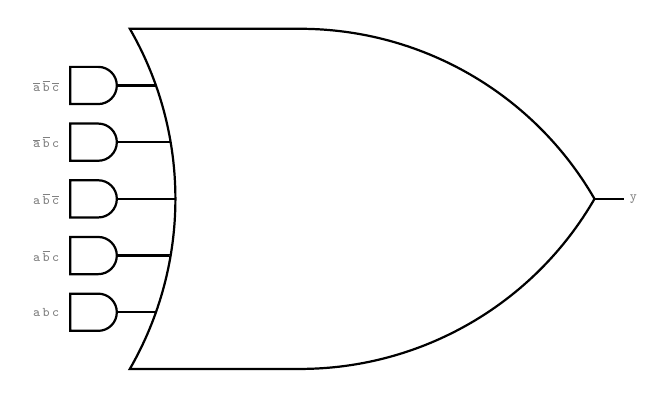
\begin{tikzpicture}[scale=0.6, transform shape]
  \node[and gate US, draw, thick, logic gate inputs=nnn] (g0) at (0,2.40012) {};
  \node[and gate US, draw, thick, logic gate inputs=nnn] (g1) at (0,1.20005) {};
  \node[and gate US, draw, thick, logic gate inputs=nnn] (g4) at (0,0) {};
  \node[and gate US, draw, thick, logic gate inputs=nnn] (g5) at (0,-1.20005) {};
  \node[and gate US, draw, thick, logic gate inputs=nnn] (g7) at (0,-2.40012) {};
  \node[left=1mm of g0, smallgraytext] {$\overline{\ttab{a}}\,\overline{\ttab{b}}\,\overline{\ttab{c}}$};
  \node[left=1mm of g1, smallgraytext] {$\overline{\ttab{a}}\,\overline{\ttab{b}}\,\ttab{c}$};
  \node[left=1mm of g4, smallgraytext] {$\ttab{a}\,\overline{\ttab{b}}\,\overline{\ttab{c}}$};
  \node[left=1mm of g5, smallgraytext] {$\ttab{a}\,\overline{\ttab{b}}\,\ttab{c}$};
  \node[left=1mm of g7, smallgraytext] {$\ttab{a}\,\ttab{b}\,\ttab{c}$};
  \node[or gate US, draw, thick, logic gate inputs=nnnnn, minimum height=7.2cm] (o) at (5,0) {};
  \draw[thick] (g0.output) -| (o.input 1);
  \draw[thick] (g1.output) -| (o.input 2);
  \draw[thick] (g4.output) -| (o.input 3);
  \draw[thick] (g5.output) -| (o.input 4);
  \draw[thick] (g7.output) -| (o.input 5);
  \draw[thick] (o.output) -- ++(0.6,0) node[right, smallgraytext] {\ttab{y}};
\end{tikzpicture}
\end{figure}
\end{frame}

\begin{frame}
  This approach works, but it is rarely the smallest circuit. Fewer terms means fewer gates, less space, and less delay.\\[3mm]
  \\
  We want a systematic way to find a small expression.
\end{frame}

% ------------------------------------------------------------
% karnaugh maps
% ------------------------------------------------------------
\begin{frame}{Karnaugh Maps}
  \begin{center}
    \Large \highlight{\textbf{Karnaugh maps}}
  \end{center}
\end{frame}
\begin{frame}
  A \highlight{\textbf{Karnaugh map}} rewrites the truth table as a grid. Neighbouring cells differ in exactly one input, so their column labels follow a special order.\\[4mm]
  \begin{figure}
  \hspace{-0.7cm}
    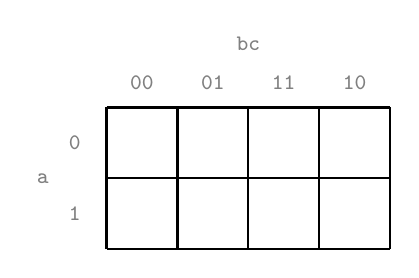
\begin{tikzpicture}[scale=0.9]
      \draw[thick] (0,0) grid (4,2);
      \foreach \x/\l in {0.5/00, 1.5/01, 2.5/11, 3.5/10}
        \node[smallgraytext] at (\x,2.35) {\ttab{\l}};
      \node[smallgraytext] at (-0.45,1.5) {\ttab{0}};
      \node[smallgraytext] at (-0.45,0.5) {\ttab{1}};
      \node[smallgraytext] at (2,2.9) {\ttab{bc}};
      \node[smallgraytext] at (-0.9,1) {\ttab{a}};
    \end{tikzpicture}
  \end{figure}
  \vspace{1mm}
  \begin{center}
    \graytext{the columns step \ttab{00}, \ttab{01}, \ttab{11}, \ttab{10}, changing one bit at a time}
  \end{center}
\end{frame}

\begin{frame}
  We fill each cell with the output for that input.
  \begin{figure}
  \hspace{-0.7cm}
    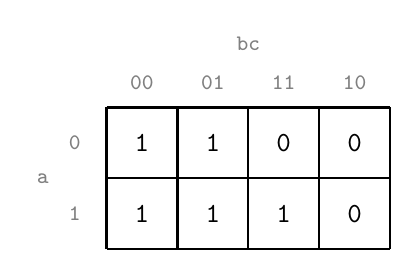
\begin{tikzpicture}[scale=0.9]
      \draw[thick] (0,0) grid (4,2);
      \foreach \x/\l in {0.5/00, 1.5/01, 2.5/11, 3.5/10}
        \node[smallgraytext] at (\x,2.35) {\ttab{\l}};
      \node[smallgraytext] at (-0.45,1.5) {\ttab{0}};
      \node[smallgraytext] at (-0.45,0.5) {\ttab{1}};
      \node[smallgraytext] at (2,2.9) {\ttab{bc}};
      \node[smallgraytext] at (-0.9,1) {\ttab{a}};
      \foreach \x/\y/\v in {
        0.5/1.5/1, 1.5/1.5/1, 2.5/1.5/0, 3.5/1.5/0,
        0.5/0.5/1, 1.5/0.5/1, 2.5/0.5/1, 3.5/0.5/0}
        \node at (\x,\y) {\ttab{\v}};
    \end{tikzpicture}
  \end{figure}
\end{frame}

\begin{frame}
  We cover the \ttab{1}s (when using sum-of-products), or \ttab{0}s (when using product-of-sums) with as few groups as possible.
  \\~\\
  A valid group obeys three rules:\\[3mm]
  \begin{itemize}
    \item it is a rectangle of \ttab{1}s (or \ttab{0}s) \\[1.5mm]
    \item its size is a power of two \\[1.5mm]
    \item it may overlap other groups and may wrap around the edges
  \end{itemize}
\end{frame}


\begin{frame}
  We circle the largest groups of adjacent \ttab{1}s (when using a sum-of-products) or \ttab{0}s (when using product-of-sums) whose size is a power of two. Each group becomes one term.\\[2mm]
  \begin{figure}
  \hspace{-0.7cm}
    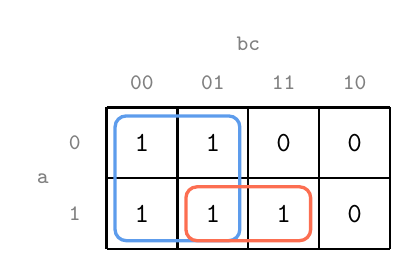
\begin{tikzpicture}[scale=0.9]
      \draw[thick] (0,0) grid (4,2);
      \foreach \x/\l in {0.5/00, 1.5/01, 2.5/11, 3.5/10}
        \node[smallgraytext] at (\x,2.35) {\ttab{\l}};
      \node[smallgraytext] at (-0.45,1.5) {\ttab{0}};
      \node[smallgraytext] at (-0.45,0.5) {\ttab{1}};
      \node[smallgraytext] at (2,2.9) {\ttab{bc}};
      \node[smallgraytext] at (-0.9,1) {\ttab{a}};
      \foreach \x/\y/\v in {
        0.5/1.5/1, 1.5/1.5/1, 2.5/1.5/0, 3.5/1.5/0,
        0.5/0.5/1, 1.5/0.5/1, 2.5/0.5/1, 3.5/0.5/0}
        \node at (\x,\y) {\ttab{\v}};
      % group of four: columns 00,01 both rows -> b bar
      \draw[very thick, myblue, rounded corners=4pt] (0.12,0.12) rectangle (1.88,1.88);
      % group of two: bottom row columns 01,11 -> a c
      \draw[very thick, myorange, rounded corners=4pt] (1.12,0.12) rectangle (2.88,0.88);
    \end{tikzpicture}
  \end{figure}
  \begin{center}
    $\ttab{y} = \overline{\ttab{b}} + \ttab{a}\ttab{c}$
  \end{center}
\end{frame}

\begin{frame}
  A group may also wrap around the edges of the map.\\[2mm]
  \begin{figure}
  \hspace{-0.7cm}
    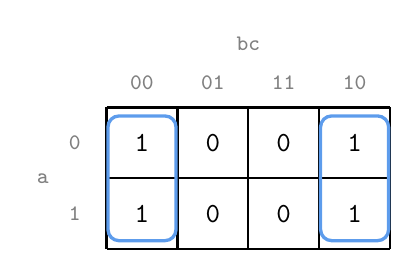
\begin{tikzpicture}[scale=0.9]
      \draw[thick] (0,0) grid (4,2);
      \foreach \x/\l in {0.5/00, 1.5/01, 2.5/11, 3.5/10}
        \node[smallgraytext] at (\x,2.35) {\ttab{\l}};
      \node[smallgraytext] at (-0.45,1.5) {\ttab{0}};
      \node[smallgraytext] at (-0.45,0.5) {\ttab{1}};
      \node[smallgraytext] at (2,2.9) {\ttab{bc}};
      \node[smallgraytext] at (-0.9,1) {\ttab{a}};
      \foreach \x/\y/\v in {
        0.5/1.5/1, 1.5/1.5/0, 2.5/1.5/0, 3.5/1.5/1,
        0.5/0.5/1, 1.5/0.5/0, 2.5/0.5/0, 3.5/0.5/1}
        \node at (\x,\y) {\ttab{\v}};
      % left edge column
      \draw[very thick, myblue, rounded corners=4pt] (0.02,0.12) rectangle (0.98,1.88);
      % right edge column
      \draw[very thick, myblue, rounded corners=4pt] (3.02,0.12) rectangle (3.98,1.88);
    \end{tikzpicture}
  \end{figure}
  \begin{center}
    \graytext{the leftmost and rightmost columns are neighbours, so together they count as a single group}
  \end{center}
\end{frame}
\begin{frame}
  Larger maps work the same way.
  \begin{figure}
  \hspace{-0.7cm}
    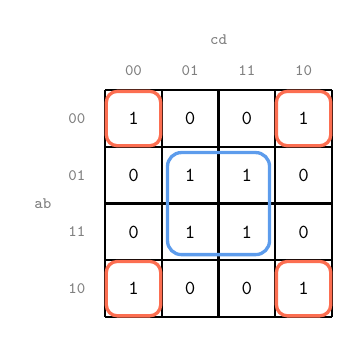
\begin{tikzpicture}[scale=0.72, transform shape]
      \draw[thick] (0,0) grid (4,4);
      \foreach \x/\l in {0.5/00, 1.5/01, 2.5/11, 3.5/10}
        \node[smallgraytext] at (\x,4.35) {\ttab{\l}};
      \foreach \y/\l in {3.5/00, 2.5/01, 1.5/11, 0.5/10}
        \node[smallgraytext] at (-0.5,\y) {\ttab{\l}};
      \node[smallgraytext] at (2,4.9) {\ttab{cd}};
      \node[smallgraytext] at (-1.1,2) {\ttab{ab}};
      \foreach \x/\y/\v in {
        0.5/3.5/1, 1.5/3.5/0, 2.5/3.5/0, 3.5/3.5/1,
        0.5/2.5/0, 1.5/2.5/1, 2.5/2.5/1, 3.5/2.5/0,
        0.5/1.5/0, 1.5/1.5/1, 2.5/1.5/1, 3.5/1.5/0,
        0.5/0.5/1, 1.5/0.5/0, 2.5/0.5/0, 3.5/0.5/1}
        \node at (\x,\y) {\ttab{\v}};
      % central block of ones (b=1, d=1)
      \draw[very thick, myblue, rounded corners=5pt] (1.1,1.1) rectangle (2.9,2.9);
      % four corners (b=0, d=0), wraps both edges
      \draw[very thick, myorange, rounded corners=4pt] (0.02,0.02) rectangle (0.98,0.98);
      \draw[very thick, myorange, rounded corners=4pt] (3.02,0.02) rectangle (3.98,0.98);
      \draw[very thick, myorange, rounded corners=4pt] (0.02,3.02) rectangle (0.98,3.98);
      \draw[very thick, myorange, rounded corners=4pt] (3.02,3.02) rectangle (3.98,3.98);
    \end{tikzpicture}
  \end{figure}
  \begin{center}
    \graytext{the four corners are all neighbours here, wrapping both the rows and the columns}
  \end{center}
\end{frame}
\end{document}
